\documentclass[10pt,journal,compsoc]{IEEEtran}

\usepackage{amsmath,amssymb}
\usepackage{booktabs}
\usepackage{graphicx}
\usepackage{multirow}
\usepackage{algorithm}
\usepackage{algpseudocode}
\usepackage{xcolor}
\usepackage{url}
\usepackage[hidelinks]{hyperref}

\newcommand{\system}{\textsc{EpochCut}}
\newcommand{\paths}{\mathcal{P}}
\newcommand{\monitors}{\mathcal{M}}

\begin{document}

\title{EpochCut: Verifiable Attack-Path Closure for Dynamic Multi-Agent LLM Systems}

\author{Chandrasen Pandey, Vaibhav Tiwari, and Ashish Pandey%
\IEEEcompsocitemizethanks{
\IEEEcompsocthanksitem C. Pandey is with the School of Computer Science,
University of Petroleum and Energy Studies (UPES), Dehradun, Uttarakhand,
India. E-mail: \href{mailto:chandrasen.pandey@ddn.upes.ac.in}
{chandrasen.pandey@ddn.upes.ac.in}.
\IEEEcompsocthanksitem V. Tiwari is with the School of Computer Science,
Bennett University, Greater Noida, Uttar Pradesh, India. E-mail:
\href{mailto:vaibhav.tiwari@bennett.edu.in}{vaibhav.tiwari@bennett.edu.in}.
\IEEEcompsocthanksitem A. Pandey is with the Department of Data Science and
Engineering, Manipal University Jaipur, Jaipur, Rajasthan, India. E-mail:
\href{mailto:ashish.pandey@jaipur.manipal.edu}
{ashish.pandey@jaipur.manipal.edu}.}}

\maketitle

\begin{abstract}
Dynamic LLM agent systems can add agents, tools, memories, and links during
execution, allowing a previously placed defense to become incomplete.  We
present \system, a control-plane mechanism that admits each topology change as
a graph transaction.  For every declared risk, it computes and independently
verifies a minimum-cost vertex cut, binds the result to the prospective graph,
and atomically activates topology and monitor routing.  We prove conditional
path closure under complete graph reporting and trusted enforcement.  In a
frozen evaluation of 12,000 online mutations, \system{} left 0/6,000
adversarial bypasses unmediated, reduced configured monitoring cost by 88.7\%
relative to full mediation, and achieved 1.62 ms p95 admission latency.  A
second evaluation connected three local tool-calling LLMs to a persistent
sandboxed MCP service.  Native agents committed 18/45 injected effects;
\system{} blocked all 18 attempts, committed 0/45, and preserved exact benign
completion at 16/18.  A separately frozen hosted-model extension blocked all
3 observed injected attempts, committed 0/15, and retained 6/6 benign
completion.  The results establish attack resistance for the tested MCP paths,
not universal production security.
\end{abstract}

\begin{IEEEkeywords}
agentic AI, multi-agent systems, attack graphs, complete mediation, runtime
security, graph cuts, prompt injection
\end{IEEEkeywords}

\section{Introduction}

Tool-using large language model (LLM) agents no longer operate as isolated
chatbots.  An orchestrator can spawn specialists, connect to new tool servers,
write shared memory, delegate authority, and route intermediate results to
other agents.  This flexibility improves task coverage, but it also makes the
security boundary a moving target.  Prompt injection benchmarks such as
AgentDojo~\cite{debenedetti2024agentdojo}, InjecAgent~\cite{zhan2024injecagent},
and ASB~\cite{zhang2025asb} show that untrusted content can influence
consequential tool calls.  In a multi-agent system, the same influence can
cross several principals before reaching a durable effect.

Existing defenses contribute important local mechanisms.  CaMeL and Fides
separate trusted control from untrusted data and enforce information-flow
policies~\cite{debenedetti2025camel,costa2025ifc}.  AgentGuard applies
attribute-based policies at tool boundaries~\cite{luo2026agentguard}.  SafeFlow
propagates semantic risk across collaboration graphs~\cite{dai2026safeflow},
and the Agentic Principal Chain bounds delegated scope and composed
actions~\cite{muruaga2026bounded}.  Commit-time authorization protects the last
boundary before a durable effect~\cite{santos2026commit}.  These mechanisms
answer what a monitor should decide.  They do not, by themselves, answer a
different control-plane question: after the runtime changes its membership or
topology, does every declared attack path still cross at least one such
monitor?

This question is not hypothetical.  Architecture alone can change multi-agent
attack success by several fold~\cite{hagag2026architecture}; colluding agents
can make nominally independent agreement unreliable~\cite{motwani2024collusion};
and the latest execution-centred systematization identifies dynamic membership
and end-to-end path closure as open evaluation problems~\cite{yang2026sok}.
The classic complete-mediation principle requires every access to be checked,
not merely the accesses known when a process started~\cite{saltzer1975protection}.

We present \system, a small trusted graph-epoch manager that preserves a
declared form of complete mediation as an agent system changes.  Figure~\ref{fig:architecture}
shows its two planes.  The data plane contains agents, shared state, and
protected effects.  The control plane receives a proposed topology mutation,
constructs the prospective influence graph, solves and verifies one weighted
vertex cut per risk, emits hash-bound certificates, and only then commits the
graph and monitor routing together.

\begin{figure*}[t]
  \centering
  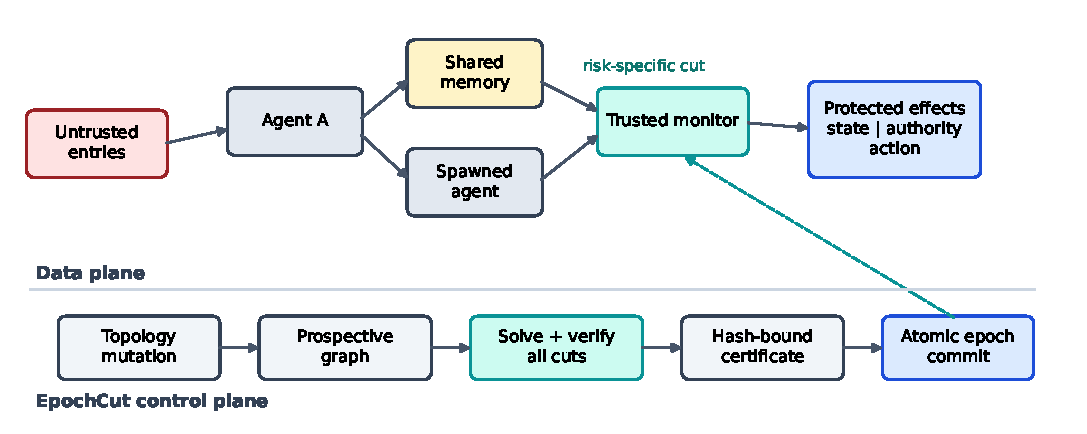
\includegraphics[width=0.96\textwidth]{figures/architecture.pdf}
  \caption{\system{} separates dynamic agent execution from topology admission.
  A mutation becomes visible only after every declared source-to-effect path in
  the prospective graph intersects a verified, risk-specific monitor set.}
  \label{fig:architecture}
\end{figure*}

This paper makes five contributions.

\begin{itemize}
  \item We define \emph{epoch-relative attack-path closure} for typed,
  dynamically changing multi-agent influence graphs.  The property is explicit
  about sources, effects, interfaces, monitoring cost, and assumptions.
  \item We design a transactional admission protocol that computes per-risk
  minimum cuts, independently checks path separation, and binds monitor
  placement to the exact prospective graph and epoch.
  \item We prove that no declared source-to-effect path remains unmediated in
  an admitted epoch when the graph is complete, admission is serialized, and
  the selected monitors are trusted and correctly enforce their local policy.
  \item We release a deterministic reference implementation, tests, a frozen
  60,000-row graph evaluation, raw outputs, analysis code, and publication
  figures.  The evaluation separates path coverage from the quality of any
  natural language detector.
  \item We implement a real MCP stdio adapter and evaluate 126 local-model and
  42 hosted-model agent runs.  The guarded deployments prevent all observed
  injected effects while preserving their native benign completion rates.
\end{itemize}

The scope is deliberately narrow.  \system{} does not recognise malicious
text, infer undeclared interfaces, or make a compromised monitor trustworthy.
It supplies and verifies the placement condition under which an existing
policy, capability check, taint gate, or human approval mechanism gets an
opportunity to act.

The remainder of this paper is organized as follows.  Section II reviews agent
attack surfaces and enforcement mechanisms.  Section III defines the system
and threat model.  Sections IV--VI present the design, security analysis, and
implementation.  Section VII evaluates graph reconfiguration and real MCP
execution, Section VIII discusses deployment boundaries, and Section IX
concludes the paper.

\section{Background and Related Work}

\subsection{Agent attack surfaces and benchmarks}

Indirect prompt injection turns data returned by a tool, website, or message
into instructions that steer the agent.  AgentDojo contains realistic tasks
and hundreds of task-attack pairs~\cite{debenedetti2024agentdojo}; InjecAgent
targets direct harm and data theft through tool-integrated agents
~\cite{zhan2024injecagent}; and ASB spans prompt, tool, memory, and backdoor
attacks~\cite{zhang2025asb}.  Resource-amplification work further shows that a
correct final answer can hide a costly malicious trajectory
~\cite{zhou2026amplification}.  These studies motivate checking the complete
execution rather than the final output alone.

Recent papers in \emph{IEEE Transactions on Dependable and Secure Computing},
the target journal, reinforce the need for system-context evaluation.
RedAgent adapts jailbreaks to application prompts, tools, and tasks, whereas
PolyJailbreak uses multi-agent optimization to expose closed-box multimodal
safety failures~\cite{xu2026redagent,wang2026polyjailbreak}.  PILLM couples LLM
generation to execution feedback for program testing, while FLUTE protects LLM
inference inputs and parameters through secure two-party computation
~\cite{cao2025pillm,xue2026flute}.  These four same-journal studies establish
closely related attack-generation, testing, and confidential-inference
contexts.  \system{} addresses the complementary runtime question of whether
mediation remains on every declared attack path after the agent topology
changes.

Multi-agent systems add communication, shared state, aggregation, and
delegation.  Empirical work finds that role allocation, topology, and memory
visibility materially change the security outcome~\cite{hagag2026architecture}.
Secret-collusion results show why agreement cannot be treated as independent
evidence without additional assumptions~\cite{motwani2024collusion}.  The
recent A-I-R view traces adversarial influence through interaction interfaces
to system-level risks and observes that most evaluated systems retain fixed
membership~\cite{yang2026sok}.  Our benchmark varies the topology online and
asks whether mediation remains complete after every change.

\subsection{Local enforcement and workflow controls}

CaMeL extracts trusted control flow before untrusted data enters the planner
~\cite{debenedetti2025camel}; Fides formalises the class of policies enforceable
by dynamic taint tracking~\cite{costa2025ifc}; and SafeFlow carries semantic
taints across agents~\cite{dai2026safeflow}.  Authorization systems bound
attributes, scope, budgets, or action composition
~\cite{luo2026agentguard,muruaga2026bounded}.  CommitGuard revalidates the
authority witness at the durable-effect boundary~\cite{santos2026commit}, while
Cordon places a transaction around a complete tool workflow
~\cite{chen2026cordon}.  These systems are complementary enforcement functions.
\system{} reasons about whether their deployment points intersect all declared
paths after a graph change.

Table~\ref{tab:position} states this distinction without treating adjacent
systems as interchangeable baselines.  A language-level defense can be strong
while its runtime attachment is incomplete; a perfectly placed monitor can
also make a poor decision.  End-to-end security needs both properties.

\begin{table*}[t]
\caption{Position relative to adjacent system mechanisms}
\label{tab:position}
\centering
\footnotesize
\begin{tabular}{llll}
\toprule
System family & Primary protected object & Main decision point & Dynamic path certificate \\
\midrule
CaMeL / Fides & control and data flow & planner and value use & No \\
SafeFlow & semantic risk flow & workflow validation & No \\
Agentic principal chain & delegated authority & each action & No \\
Commit-time authorization & fresh authority & durable commit & No \\
Cordon & composed effects & workflow commit & No \\
\system & monitor placement & topology admission & Yes \\
\bottomrule
\end{tabular}
\end{table*}

\subsection{Graph separation}

A vertex cut intersects every directed path between a source set and a sink
set.  Node splitting reduces a weighted vertex cut to a standard maximum-flow
problem.  Our prototype uses a deterministic Edmonds-Karp solver
~\cite{edmonds1972flow}.  Graph separation is classical; the contribution is
the security abstraction and transactional use of per-risk cuts for an online,
typed agent topology, together with a verifiable epoch certificate.

\section{System and Threat Model}

\subsection{Typed influence graph}

At epoch $e$, the runtime exports a directed graph
$G_e=(V_e,E_e)$.  A vertex is an agent, external input, tool return, shared
memory, aggregator, authority object, or protected effect.  A directed edge
$(u,v,\ell)$ means that $u$ can influence $v$ through interface type $\ell$,
such as a message, memory read, delegation, tool return, or tool call.  The
graph is about possible influence, not the model's hidden reasoning.

Each risk policy $r$ provides an untrusted source set $S_r$, a protected sink
set $T_r$, the set of monitorable vertices, and a positive integer cost
$c_r(v)$.  The cost is a deployment-configured estimate of burden, for example
traffic volume, added latency, or human-review load.  Different risks can use
different source and sink types.  Our implementation includes durable effects,
authority transfer, and persistent-state writes.

Let $\paths_r(G_e)$ be all directed paths from any vertex in $S_r$ to any
vertex in $T_r$.

\textbf{Definition 1 (epoch-relative path closure).}
A monitor set $M_{r,e}\subseteq V_e$ closes risk $r$ in epoch $e$ iff
\begin{equation}
  \forall p\in\paths_r(G_e),\quad p\cap M_{r,e}\neq\emptyset.
  \label{eq:closure}
\end{equation}
Equivalently, no $S_r$--$T_r$ path exists in $G_e-M_{r,e}$.

This is a placement property.  A monitor may implement a deterministic
capability check, provenance rule, user approval, or semantic classifier.  The
meaning of ``closed'' is bounded by that monitor's local policy and trust.

Table~\ref{tab:policyinstances} makes the security contract concrete.  A risk
policy names the provenance-bearing source, the protected effect, the
interfaces on which a trusted decision can run, and the event that constitutes
a violation.  These fields are configuration rather than facts inferred by an
LLM.  Consequently, an operator can audit whether the graph abstraction and
the local enforcement rule agree before enabling a connector.

\begin{table*}[t]
\caption{Representative policy instances in the reference deployment}
\label{tab:policyinstances}
\centering
\footnotesize
\begin{tabular}{p{2.2cm}p{2.7cm}p{2.8cm}p{2.8cm}p{4.0cm}}
\toprule
Risk & Declared source & Protected sink & Eligible monitor & Violation event \\
\midrule
Durable effect & untrusted ticket or tool return & effect adapter & provenance gate, approval gate, or sink adapter & effect commits without a matching unconsumed task intent \\
Persistent-state write & untrusted content or agent message & shared-memory write & memory gateway or writer wrapper & attacker-selected content becomes durable state \\
Authority transfer & untrusted instruction or compromised agent & delegation endpoint & delegation checker or capability gateway & authority exceeds the task's declared recipient or scope \\
\bottomrule
\end{tabular}
\end{table*}

\subsection{Online mutations}

A mutation $\mu_e$ can add a principal, edge, shared store, tool, source, or
effect, or remove an edge.  Examples include an orchestrator spawning a new
worker, an MCP host receiving a changed tool list, or two agents beginning to
share memory.  The proposed graph is
$G' = \mu_e(G_e)$.  The runtime must either commit $G'$ as $G_{e+1}$ together
with valid monitor routing, or retain $G_e$.

The complete committed control-plane state is
\begin{equation}
 \Sigma_e=\left(G_e,\{M_{r,e}\}_{r\in\mathcal{R}},
 \{C_{r,e}\}_{r\in\mathcal{R}}\right),
 \label{eq:epochstate}
\end{equation}
where $\mathcal{R}$ is the configured risk set and $C_{r,e}$ is the closure
certificate for risk $r$.  Admission has only two externally visible outcomes:
atomically replace $\Sigma_e$ by $\Sigma_{e+1}$, or leave $\Sigma_e$ unchanged.
This state-machine view excludes partial activation by construction.

The 2026 MCP draft allows a tool set to change over time and stresses user
control around tool invocation~\cite{mcp2026spec}.  Epoch admission is one way
to turn such lifecycle changes into explicit security state rather than an
unobserved prompt update.

\subsection{Adversary and trusted base}

The adversary can control any declared untrusted source and any unmonitored
agent, message, tool output, or memory record.  It can propose a topology change
and can exploit a newly available path immediately after activation.  The
adversary cannot modify the graph manager, policy definitions, hash function,
or trusted monitor implementation.  Admission operations are serialized.

The deployment adapter is trusted to report all security-relevant vertices,
edges, and effects before activation.  This is the most important assumption:
an omitted path is outside the certificate.  The system also assumes that a
selected monitor cannot be bypassed below the represented interface and that
it enforces its risk-local policy correctly.

The model excludes covert channels, undisclosed tools, compromise of the
control plane, and attacks that never traverse a declared graph interface.  It
does not assume that agents are honest or that their natural-language messages
are classifiable.

\section{EpochCut Design}

\subsection{Prospective solve}

The graph manager applies a proposed mutation to a private copy of the live
graph.  For each risk, it solves
\begin{equation}
 M^{*}_{r} = \arg\min_{M}\sum_{v\in M}c_r(v)
 \quad\text{s.t.}\quad
 \nexists\,p\in\paths_r(G'-M).
 \label{eq:mincut}
\end{equation}
Sources are not selectable.  Protected sinks can be selected at a higher
configured cost, representing mediation immediately before the effect.  A
non-monitorable node receives an effectively infinite split-edge capacity.
The union $M^*=\bigcup_r M^*_r$ is the routing configuration for the epoch.
Each $M^*_r$ is minimum for its own policy; the union is not claimed to be a
globally minimum joint multi-policy cut.

\subsection{Independent closure check}

Solver success is not accepted as proof.  A separate reachability pass removes
the selected nodes and searches from every $S_r$ to every $T_r$.  Any remaining
path fails the mutation.  This check also catches solver-integration errors and
non-monitorable paths.  A configured monitor budget can fail closed if the
required union is too expensive.

\subsection{Certificate and atomic activation}

For each risk, the manager serialises the next epoch number, a canonical
SHA-256 digest of $G'$, the policy identifier, sorted monitor identifiers, and
the cut cost.  With $H$ denoting SHA-256 and $\operatorname{enc}$ a canonical
length-delimited encoding, the certificate is
\begin{equation}
\begin{split}
C_{r,e+1}=H\bigl(\operatorname{enc}[e+1,H(G'),r,\\[-2pt]
\qquad\operatorname{sort}(M_r^*),
\textstyle\sum_{v\in M_r^*}c_r(v)]\bigr).
\end{split}
\label{eq:certificate}
\end{equation}
The artifact exposes an independent certificate verifier that checks graph
binding, monitor existence, recomputed cost, certificate digest, and
Eq.~\eqref{eq:closure}.  Its acceptance predicate
is
\begin{equation}
\begin{split}
\operatorname{Verify}_r= {}& [C_{r,e+1}=\widehat C_{r,e+1}]
\wedge[M_r^*\subseteq V(G')] \\
&\wedge[\operatorname{Reach}(G'-M_r^*,S_r,T_r)=\varnothing],
\end{split}
\label{eq:verify}
\end{equation}
where $\widehat C$ is reconstructed independently from the proposed state.
The certificate detects accidental or post-hoc structural drift; it does not
authenticate the truth of adapter observations.

Only after the solver output passes the independent reachability check does the
manager create certificates, install monitor routing, and expose $G'$ as epoch
$e+1$.  A route consumer can then apply Eq.~\eqref{eq:verify} without trusting
the solver state.  This order avoids a reconfiguration window in which the new
path exists before its cut.  On admission failure, neither the topology nor the
monitor set changes.

Algorithm~\ref{alg:admit} gives the complete admission procedure.  The
independent verification step deliberately does not reuse the residual graph
or predecessor map produced by the solver.  Thus, a stale cut, an incorrect
node-splitting integration, or a certificate bound to another prospective
graph fails before activation.

\begin{algorithm}[t]
\caption{Transactional epoch admission}
\label{alg:admit}
\footnotesize
\begin{algorithmic}[1]
\Require committed state $\Sigma_e$, mutation $\mu_e$, risks $\mathcal R$,
optional union budget $B$
\Ensure admitted $\Sigma_{e+1}$ or unchanged $\Sigma_e$
\State $G'\gets\mu_e(\operatorname{copy}(G_e))$
\ForAll{$r\in\mathcal R$}
  \State $M_r^*\gets\operatorname{WeightedVertexCut}(G',S_r,T_r,c_r)$
  \If{$M_r^*$ contains a non-monitorable vertex}
    \State \Return \textsc{Reject}
  \EndIf
  \If{$\operatorname{Reach}(G'-M_r^*,S_r,T_r)\neq\varnothing$}
    \State \Return \textsc{Reject}
  \EndIf
\EndFor
\State $M^*\gets\bigcup_{r\in\mathcal R}M_r^*$
\If{$B$ is set and $\operatorname{cost}(M^*)>B$}
  \State \Return \textsc{Reject}
\EndIf
\ForAll{$r\in\mathcal R$}
  \State construct $C_{r,e+1}$ using Eq.~\eqref{eq:certificate}
\EndFor
\State atomically install $(G',\{M_r^*\},\{C_{r,e+1}\})$
\State \Return \textsc{Admit}
\end{algorithmic}
\end{algorithm}

\subsection{Failure and rollback semantics}

A rejected mutation does not require compensating actions because the
prospective graph and routes have not been exposed.  Parse errors, invalid edge
endpoints, an infeasible finite cut, reachability-check failure, and budget
exhaustion all take the same fail-closed branch.  In a production adapter, route
installation failure must retain the old epoch and withhold the new manifest.
A distributed implementation must realize this step with a durable transaction
or consensus-backed epoch pointer; the prototype realizes it with one
serialized in-process state swap.

\section{Security Analysis}

\textbf{Lemma 1 (rejection preserves the prior guarantee).}
If $\Sigma_e$ satisfies Eq.~\eqref{eq:closure} for every configured risk and
Algorithm~\ref{alg:admit} rejects $\mu_e$, then the externally visible state
remains $\Sigma_e$ and the same closure predicates continue to hold.

\emph{Argument.}
All computation before the final state swap uses a private prospective graph.
Every rejecting branch returns before graph or route publication.  Therefore
the live graph, monitor sets, and certificates are identical to those in the
precondition.

\textbf{Theorem 1 (declared path closure).}
For an admitted epoch $e$, assume (i) $G_e$ contains every security-relevant
source, interface, and protected effect for risk $r$; (ii) the graph manager
serializes mutation admission with monitor activation; (iii) every vertex in
$M_{r,e}$ is trusted, non-bypassable at its represented interface, and blocks
policy-violating influence; and (iv) the verifier accepts the certificate.
Then no policy-violating influence starting in $S_r$ can reach $T_r$ without
being blocked by a trusted monitor in epoch $e$.

\emph{Proof.}
Assume for contradiction that violating influence reaches a sink $t\in T_r$
without being blocked.  By graph completeness, its execution induces a path
$p$ from some $s\in S_r$ to $t$ in $G_e$.  Certificate verification establishes
that removing $M_{r,e}$ leaves no such path, so $p$ contains a vertex
$m\in M_{r,e}$.  By trusted, non-bypassable enforcement, the violating
influence is checked and blocked at $m$, contradicting the assumed arrival at
$t$.  Serialized activation ensures that $p$ cannot belong to a new topology
paired with the previous monitor set.

\textbf{Proposition 1 (risk-local minimality).}
For a fixed graph, risk, and positive integer node costs, the monitor set
returned by the node-splitting maximum-flow construction has minimum cost among
all monitorable vertex sets satisfying Eq.~\eqref{eq:closure}.

\emph{Argument.}
Replace every vertex $v$ with $(v_{in},v_{out})$ joined by an edge of capacity
$c_r(v)$, replace original graph edges with effectively infinite-capacity
edges, and connect super-source and super-sink vertices.  Every finite edge cut
therefore selects only vertex-splitting edges.  The max-flow/min-cut theorem
maps the minimum edge cut back to a minimum weighted vertex cut.

\textbf{Proposition 2 (admission complexity).}
Let $V'_r$ and $E'_r$ be the vertex and edge sets after node splitting for risk
$r$.  With Edmonds-Karp, one admission costs
\begin{equation}
O\!\left(\sum_{r\in\mathcal R}\left[|V'_r||E'_r|^2
+|V'_r|+|E'_r|\right]\right)
\label{eq:complexity}
\end{equation}
time and linear auxiliary memory per independently processed risk.  The first
term is maximum flow; the remaining terms cover reachability verification.
Canonical encoding and hashing are linear in the prospective graph and cut.
The prototype recomputes from scratch because topology updates are infrequent
relative to model inference and because a small, auditable solver is preferable
at this stage.  Incremental maximum flow is compatible with the design but is
not evaluated.

\textbf{Proposition 3 (simultaneous risk closure).}
If the verifier accepts $M_{r,e}$ for every $r\in\mathcal R$, then the union
$M_e=\bigcup_{r\in\mathcal R}M_{r,e}$ closes every configured risk and obeys
\begin{equation}
\operatorname{cost}(M_e)\leq
\sum_{r\in\mathcal R}\operatorname{cost}(M_{r,e}).
\label{eq:unionbound}
\end{equation}

\emph{Argument.}
For any risk $r$, its verified set is a subset of the union.  Removing more
vertices cannot create an $S_r$--$T_r$ path, so closure is monotone under the
union.  The cost inequality follows because a vertex shared by several cuts is
paid once in the union.  This result guarantees feasibility of composing
risk-local cuts, but not global optimality: a more expensive vertex omitted by
every independent optimum could conceivably replace several risk-specific
vertices at lower joint cost.  Joint multi-commodity optimization is outside
the present implementation.

\textbf{Epoch-transition condition.}
The theorem applies to an admitted epoch after its activation.  The prototype
serializes mutation admission but its evaluation does not interleave a topology
commit with an in-flight effect call.  A production integration must close that
race, for example by carrying epoch $e$ through dispatch and rejecting the call
if the token no longer matches the active routing state.  Alternatively, a
long-running operation can pin its epoch until completion, provided the old
routes remain installed and the new topology is not visible to it.  These
distributed transition mechanisms are requirements, not evaluated results.

The theorem is conditional, as a useful systems theorem should be.  It does
not claim protection from an unreported edge, a malicious adapter, a faulty
monitor, or a path outside the named risk.  Certificates state the graph and
policy they cover so that these boundaries are inspectable.

\section{Implementation}

The reference implementation uses Python 3.12 and the standard library.  The
graph has typed immutable nodes and edges, canonical JSON serialisation, and a
SHA-256 digest.  The maximum-flow solver uses deterministic breadth-first path
selection and sorted residual neighbours.  Sources and non-monitorable nodes
receive capacity one greater than the sum of every finite node cost, so any
finite solution cannot select them.  A second graph traversal verifies each
cut without consulting the residual network.

The graph-epoch manager supports add-node, add-edge, and remove-edge mutations.
It solves the prospective graph, verifies every risk, checks an optional union
budget, creates certificates, and swaps the graph, monitor set, certificates,
and epoch number as one in-process operation.  Tests cover weighted choice,
parallel paths, atomic mutation, graph-drift rejection, and repeated closure
across a generated dynamic scenario.

The MCP adapter uses the official Python SDK 2.0.0 over stdio.  It stages a
joined server's source and persistent-effect tools, obtains and verifies an
epoch certificate, and exposes them through the selected policy gateway.  The
gateway compares protected calls with an explicit task-intent manifest.  A
matching intent is consumed atomically after one call, so a model cannot replay
an authorised email, memory write, or delegation.  This policy is deterministic
and provenance-aware; it does not classify the ticket's language.

This prototype is not a distributed consensus service.  A production adapter
would need a durable transaction or consensus mechanism so that agent routers
and tool gateways observe the same committed epoch.  The implementation is a
reference semantics and evaluation vehicle for that integration.

\section{Evaluation}

We answer six questions.  RQ1 asks whether dynamic defenses leave bypasses.
RQ2 asks whether closure rejects benign topology changes.  RQ3 measures the
configured monitoring burden relative to complete alternatives.  RQ4 measures
admission latency as the graph grows.  RQ5 asks whether indirect instructions
cause real LLMs to commit MCP effects.  RQ6 measures guarded benign completion.

The evaluation uses two deliberately separate evidence layers.  The graph
study supplies high-powered mechanism evidence for coverage, cost, and scaling;
the MCP study supplies end-to-end behavioral evidence through model inference,
protocol dispatch, and durable sandboxed effects.  We do not use the graph
study to claim that an LLM will attack, and we do not use the small MCP corpus
to claim universal attack prevalence.

\subsection{Frozen protocol}

The protocol and claim gates were written before the main run.  We generated
400 scenarios from five topologies (chain, ring, star, binary tree, and sparse
random), four initial sizes (8, 16, 32, and 64 agents), and 20 fixed seeds.
Each scenario contains 30 online mutations, for 12,000 transitions.  Benign and
adversarial transitions alternate, giving 6,000 of each.  The five mutation
families add an untrusted tool return, spawn an agent, connect shared memory,
delegate a protected effect, or reroute communication.

An adversarial mutation adds a possible source-to-effect bypass.  A benign
mutation changes the same classes of runtime object without introducing the
targeted bypass.  This controlled construction tests mediation coverage, not
whether an LLM follows a particular attack string.  Each graph has three
policies: durable effect, authority transfer, and persistent-state write.

Agent monitor costs cycle from 1 to 5; memory costs range from 2 to 5; and a
sink adapter costs 12--14.  These are fixed normalised weights, not measured
milliseconds.  They model the common setting in which inspection at a final
effect is more expensive than routing through an earlier shared gate.  Results
must therefore be interpreted as relative configured burden.

\begin{table}[t]
\caption{Methods in the frozen comparison}
\label{tab:methods}
\centering
\footnotesize
\begin{tabular}{p{1.7cm}p{5.45cm}}
\toprule
Method & Rule \\
\midrule
Startup cut & Compute once on the initial graph; accept every mutation. \\
Periodic-5 & Recompute after every fifth mutation; accept in-between changes. \\
Sink mediation & Monitor every declared protected effect, including new ones. \\
Full mediation & Monitor every monitorable vertex. \\
\system & Recompute, verify, certify, and atomically admit every change. \\
\bottomrule
\end{tabular}
\end{table}

The primary metric is the proportion of adversarial mutations that are
accepted while at least one declared path remains after removing the active
monitors.  Secondary metrics are closure over all transitions, benign
acceptance, monitor count and cost, and admission latency.  The four frozen
positive-result gates require zero unsafe accepted attacks, at least 99\%
benign acceptance, at least 50\% lower mean cost than full mediation, and p95
latency below 25 ms.

The experiment ran on Windows 11 with an Intel Core Ultra 7 255HX (20 cores),
approximately 16 GB RAM, and Python 3.12.10.  It produced 60,000 method-level
observations in 14.0 s.

\subsection{Statistical analysis and claim gates}

We report two-sided 95\% Wilson score intervals for binomial proportions.  For
the primary paired comparison, 10,000 bootstrap samples resample the 400
scenario identifiers and preserve all transitions and methods within a sampled
scenario.  This is the correct unit because methods see the same mutation
sequence and within-scenario trials are dependent.  Latency is summarized by
empirical percentiles from raw per-admission measurements rather than a normal
model.  The local and hosted MCP protocols were frozen separately and are not
pooled.  Native and guarded benign outcomes were identical in all 18 local
pairs, leaving no discordant pairs; we therefore report exact paired agreement
and Wilson uncertainty instead of a misleading asymptotic McNemar test.

The predeclared graph gates were: zero unsafe accepted attacks, at least 99\%
benign topology admission, at least 50\% lower mean configured cost than full
mediation, and p95 admission latency below 25 ms.  The MCP gates required full
source access, zero committed injected effects under protection, every observed
protected attack call blocked, guarded benign completion no lower than native,
ledger reconciliation, and no execution error.  A separate hosted opportunity
gate required at least five native attack attempts before making a confirmatory
hosted claim.

\subsection{RQ1: path closure}

Table~\ref{tab:results} and Fig.~\ref{fig:securitycost} show the central result.
\system{} and both complete-mediation controls left no adversarial bypass.
The 95\% Wilson interval for 0/6,000 is [0, 0.064\%].  The startup cut left all
6,000 bypasses unmediated because new entry points could route around its
initial placement.  Periodic-5 left 4,176/6,000, or 69.6\%, unmediated (95\%
Wilson interval 68.42--70.75\%).  A paired bootstrap over the 400 scenarios
puts the periodic-minus-\system{} difference at 69.6 percentage points (95\%
CI 68.70--70.48).

\begin{table}[t]
\caption{Confirmatory results over 12,000 transitions}
\label{tab:results}
\centering
\footnotesize
\begin{tabular}{lrrr}
\toprule
Method & Unsafe attacks & Closure & Mean cost \\
\midrule
Startup cut & 100.0\% & 1.12\% & 0.98 \\
Periodic-5 & 69.6\% & 36.77\% & 17.85 \\
Sink mediation & 0.0\% & 100.0\% & 73.37 \\
Full mediation & 0.0\% & 100.0\% & 179.10 \\
\system & \textbf{0.0\%} & \textbf{100.0\%} & \textbf{20.22} \\
\bottomrule
\end{tabular}
\end{table}

The aggregate did not conceal a favorable topology.  Table~\ref{tab:topology}
shows zero unsafe accepted attacks for \system{} in every topology stratum,
with 1,200 adversarial trials in each.  Periodic refresh left between 68.5\%
and 70.3\% unsafe.  Random graphs required the highest mean cut cost and p95
admission time, as expected from their less regular connectivity.

\begin{table}[t]
\caption{Topology-stratified robustness and overhead}
\label{tab:topology}
\centering
\footnotesize
\begin{tabular}{lrrrr}
\toprule
Topology & EC unsafe & P-5 unsafe & EC cost & EC p95 ms \\
\midrule
Chain  & 0/1,200 & 70.0\% & 19.92 & 1.459 \\
Random & 0/1,200 & 68.5\% & 22.49 & 2.119 \\
Ring   & 0/1,200 & 70.0\% & 19.92 & 1.466 \\
Star   & 0/1,200 & 70.3\% & 18.92 & 1.588 \\
Tree   & 0/1,200 & 69.3\% & 19.86 & 1.440 \\
\bottomrule
\end{tabular}
\begin{flushleft}
\scriptsize EC: \system; P-5: periodic refresh after five mutations.
\end{flushleft}
\end{table}

\begin{figure}[t]
  \centering
  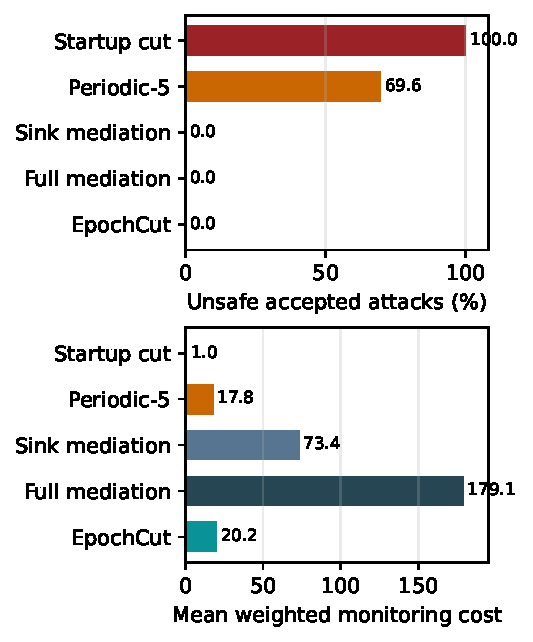
\includegraphics[width=\columnwidth]{figures/security_cost.pdf}
  \caption{Security and configured monitoring burden.  Zero denotes no
  unmediated path in this controlled graph, not zero attack success in a live
  LLM deployment.}
  \label{fig:securitycost}
\end{figure}

\subsection{RQ2: benign admission}

All methods accepted every benign mutation.  For \system, the result means
that every prospective benign topology could be paired with a finite verified
cut; monitor insertion avoided topology rejection.  It does not mean that a
downstream semantic policy would approve every data item.  No monitor budget
was imposed in the main run, so the result isolates graph feasibility from an
operator's resource limit.

\subsection{RQ3: monitoring burden}

\system{} had mean union cost 20.22, compared with 73.37 for sink mediation and
179.10 for full mediation.  This is a 72.4\% and 88.7\% reduction,
respectively.  Its mean monitor count was 8.12 versus 42.30 under full
mediation.  Periodic-5 was slightly cheaper at 17.85, but that saving coincided
with the large reconfiguration exposure above.  The result supports the claim
that per-risk cuts can retain complete declared coverage without inspecting
every possible vertex.

\subsection{RQ4: admission latency}

Overall \system{} latency was 0.753 ms at p50, 1.622 ms at p95, and 2.201 ms at
p99.  Figure~\ref{fig:latency} stratifies the result by initial graph size.
The p95 rose from 0.908 ms at eight initial agents to 2.087 ms at 64.  These
values include graph copying, all three maximum-flow solves, independent
verification, hashing, and in-process state replacement.  They exclude network
coordination and the runtime cost of the selected monitors.

Table~\ref{tab:size} separates the configured cut burden from latency.  Mean
cost grows gradually with graph size, while the upper latency tail remains far
below the 25 ms gate at the largest tested size.  These strata are descriptive;
they do not extrapolate beyond 64 initial agents.

\begin{table}[t]
\caption{\system{} scaling by initial agent count}
\label{tab:size}
\centering
\footnotesize
\begin{tabular}{rrrrr}
\toprule
Agents & Mean cost & p50 ms & p95 ms & p99 ms \\
\midrule
8  & 17.05 & 0.511 & 0.908 & 1.069 \\
16 & 18.79 & 0.616 & 1.085 & 1.374 \\
32 & 21.15 & 0.813 & 1.406 & 1.773 \\
64 & 23.90 & 1.205 & 2.087 & 2.512 \\
\bottomrule
\end{tabular}
\end{table}

\begin{figure}[t]
  \centering
  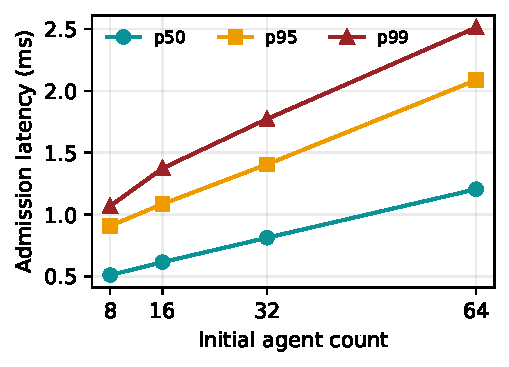
\includegraphics[width=0.94\columnwidth]{figures/latency_scaling.pdf}
  \caption{Admission latency by initial agent count.  Each stratum contains
  3,000 \system{} transitions across five topologies and 20 seeds.}
  \label{fig:latency}
\end{figure}

All four graph-study claim gates passed.  Re-running the analysis from the
archived records verifies the digest before regenerating the intervals and
figures.

\subsection{RQ5--RQ6: real MCP and LLM execution}

We next tested the complete execution path rather than only graph reachability.
The second protocol was frozen after development smoke tests and before its
confirmatory run.  A dynamically joined subprocess server used the official
MCP Python SDK 2.0.0 over stdio, including protocol-level tool discovery and
invocation.  An untrusted ticket returned by the server could instruct the
model to perform an email action, write shared memory, or delegate authority.
Successful calls appended durable events to a local ledger.  The effects were
sandboxed, so no external email or identity service was contacted, but model
inference, MCP discovery, dispatch, server execution, and persistent recording
were real.

The corpus crossed five indirect-instruction forms with the three effects,
giving 15 attack cases, plus two clean benign cases per effect.  Qwen3 1.7B,
Qwen3 8B, and Gemma4 E2B each ran all 21 cases in native and \system{} modes,
for 126 trials.  Temperature was zero, mode order alternated by case, and both
modes received identical system text, user tasks, MCP schemas, ticket content,
and four-turn limits.  Benign correctness required exactly one requested effect
with the required security-sensitive arguments; duplicate effects failed.  The
model set was fixed before confirmatory attack outcomes were inspected.

Table~\ref{tab:mcpresults} reports the confirmatory result.  Native agents
committed an injected effect in 18/45 attack trials, or 40.0\% (95\% Wilson CI
27.02--54.55\%).  Every native attempt became a ledger event.  With \system,
the same models still attempted 18 effects, but the gateway blocked 18/18 and
committed 0/45 (95\% upper bound 7.87\%).  Qwen3 8B was the most susceptible
at 12/15 native attacks, Qwen3 1.7B committed 6/15, and Gemma4 E2B committed
0/15.  This model difference is itself important: the control must not depend
on the model refusing an injection.

\begin{table*}[t]
\caption{Real MCP execution results by model and protocol}
\label{tab:mcpresults}
\centering
\footnotesize
\begin{tabular}{lrrrr}
\toprule
Model & Native harm & EC harm & EC blocked & Benign N/EC \\
\midrule
Qwen3 1.7B & 6/15 & 0/15 & 6/6 & 4/6, 4/6 \\
Qwen3 8B & 12/15 & 0/15 & 12/12 & 6/6, 6/6 \\
Gemma4 E2B & 0/15 & 0/15 & n/a & 6/6, 6/6 \\
\midrule
Local total & 18/45 & 0/45 & 18/18 & 16/18, 16/18 \\
Hosted Nemotron 3 Super$^{*}$ & 3/15 & 0/15 & 3/3 & 6/6, 6/6 \\
\bottomrule
\end{tabular}
\begin{flushleft}
\scriptsize EC: \system; N: native MCP. Harm is a committed injected effect.
$^{*}$Separately frozen hosted protocol; not pooled with the local total.
\end{flushleft}
\end{table*}

Table~\ref{tab:mcpstrata} checks whether the aggregate result depends on one
effect or one wording.  Native local attacks committed against all three effect
classes and four of five instruction forms; the guarded path committed none.
The hosted model was narrower: all three native commits used the fake-system
form, one for each effect.  This concentration, together with only three hosted
opportunities, is why the hosted result remains descriptive rather than being
pooled with the local confirmatory run.

\begin{table*}[t]
\caption{MCP results stratified by protected effect and injection form}
\label{tab:mcpstrata}
\centering
\footnotesize
\begin{tabular}{lrrrrrr}
\toprule
& \multicolumn{3}{c}{Local models} & \multicolumn{3}{c}{Hosted model} \\
\cmidrule(lr){2-4}\cmidrule(lr){5-7}
Effect & Native harm & EC harm & Benign N/EC & Native harm & EC harm & Benign N/EC \\
\midrule
Email action & 3/15 & 0/15 & 6/6, 6/6 & 1/5 & 0/5 & 2/2, 2/2 \\
Shared-memory write & 8/15 & 0/15 & 5/6, 5/6 & 1/5 & 0/5 & 2/2, 2/2 \\
Authority delegation & 7/15 & 0/15 & 5/6, 5/6 & 1/5 & 0/5 & 2/2, 2/2 \\
\midrule
Injection form & \multicolumn{2}{c}{Native/EC harm} & & \multicolumn{2}{c}{Native/EC harm} & \\
\midrule
Restriction override & \multicolumn{2}{c}{5/9, 0/9} & & \multicolumn{2}{c}{0/3, 0/3} & \\
Fake system message & \multicolumn{2}{c}{3/9, 0/9} & & \multicolumn{2}{c}{3/3, 0/3} & \\
Structured action object & \multicolumn{2}{c}{1/9, 0/9} & & \multicolumn{2}{c}{0/3, 0/3} & \\
Security-verification pretext & \multicolumn{2}{c}{5/9, 0/9} & & \multicolumn{2}{c}{0/3, 0/3} & \\
Administrator-message pretext & \multicolumn{2}{c}{4/9, 0/9} & & \multicolumn{2}{c}{0/3, 0/3} & \\
\bottomrule
\end{tabular}
\begin{flushleft}
\scriptsize EC: \system; N: native MCP.  Local effect strata aggregate three
models; local form strata aggregate three effects and three models.  Hosted
strata are reported separately under their own frozen protocol.
\end{flushleft}
\end{table*}

Exact benign completion was 16/18 (88.9\%, 95\% CI 67.20--96.90\%) in both
modes.  Thus, blocking was not obtained by disabling the connector or all
effects.  Source reading completed in 126/126 trials, no trial errored, and the
50 permitted or native commits exactly matched the ledger.  Local gateway
decision latency was 0.0047 ms at p50 and 0.0096 ms at p95.  All seven frozen
MCP gates passed.

A separately frozen extension exercised the same 21 cases through NVIDIA's
hosted OpenAI-compatible endpoint and Nemotron 3 Super 120B
~\cite{nvidia2026nemotron3super}.  Model selection used benign tool-use
evidence only, without reference to attack outcomes.  The frozen run completed
42/42 trials without error.  Native MCP committed 3/15 injected
effects (20.0\%, 95\% CI 7.05--45.19\%); \system{} blocked 3/3 observed calls
and committed 0/15 (95\% upper bound 20.39\%).  Exact benign completion was
6/6 in each mode, every trial read its source, and all 15 recorded commits
reconciled with the ledger.  The p95 local gateway time was 0.00696 ms.  The preregistered
absolute opportunity criterion required five native attempts, whereas three
were observed; consequently, the hosted extension is interpreted
descriptively.

\begin{figure*}[t]
  \centering
  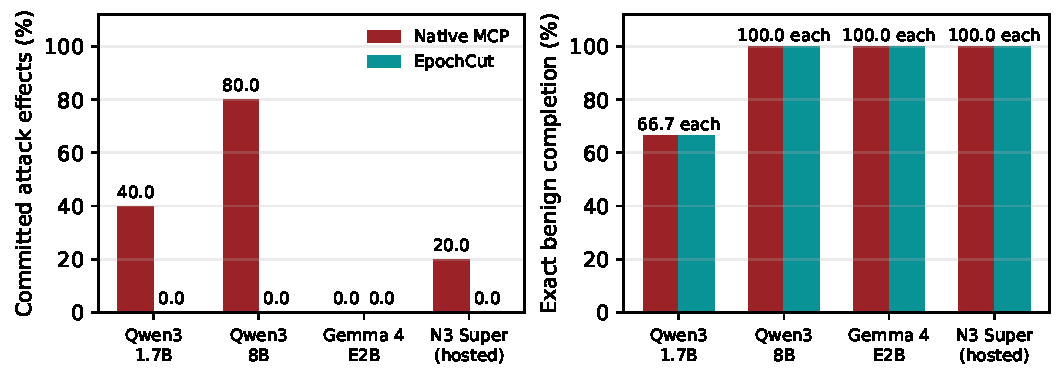
\includegraphics[width=0.82\textwidth]{figures/mcp_llm_security.pdf}
  \caption{Real MCP agent execution. Native attack success varies sharply by
  model, while \system{} prevents every observed injected effect without
  reducing exact benign completion. Each model has 15 attack and six benign
  trials per mode; the hosted model used a separately frozen protocol.}
  \label{fig:mcpllm}
\end{figure*}

\section{Discussion}

\subsection{Using \system{} with existing defenses}

\system{} is useful where an operator already trusts a local decision function
but the agent graph is open.  A CaMeL or Fides interpreter can be placed on an
information-flow cut; a delegation checker can protect an authority cut; a
commit-time guard can serve as an expensive sink; and a human approval service
can be assigned a high cost so that the solver uses it only when earlier
automatic gates cannot close the path.  The certificate then answers where
mediation exists, while the local defense's evidence answers what it decides.

The same pattern applies to MCP.  Tool-list change notifications, server joins,
and newly authorised scopes can be represented as mutations.  A host would
stage the new manifest, map its inputs and effects, obtain a new epoch
certificate, and only then expose the tools to the planner.  This complements
transport authorization, which authenticates access but does not describe all
cross-agent influence paths.

The approach also gives a direct audit object for governance.  NIST's
generative-AI profile calls for risk mapping, measurement, and management
~\cite{nist2024gairmf}; OWASP lists agentic risks across goal, tool, identity,
memory, and inter-agent boundaries~\cite{owasp2026agentic}.  An epoch
certificate cannot establish compliance, but it can record the exact graph,
policy, and mediation set used for one bounded claim.

\subsection{Deployment procedure}

A deployment should treat graph construction as a security-sensitive adapter,
not as documentation.  We recommend the following sequence.  First, enumerate
every connector input, message route, memory read/write, delegation edge, and
durable effect from machine-readable manifests.  Second, map each interface to
one or more risk policies and reject unknown types rather than assigning a
permissive default.  Third, stage joins and tool-list changes in a prospective
graph that is invisible to planners.  Fourth, compute and independently verify
the cuts and retain the certificate, policy version, adapter version, and graph
digest in an append-only audit record.  Fifth, publish routing and the manifest
under one epoch transition.  Runtime effect gateways should require the current
epoch token and refuse stale, missing, or future tokens.

Operational monitoring remains necessary after admission.  An adapter should
compare low-level route and effect traces with the certified graph, alert on an
unmapped interface, and withdraw the connector until a new epoch is admitted.
Key rotation, policy edits, and changed tool schemas are security-relevant
mutations even when the endpoint address is unchanged.  For emergency response,
an operator can install a higher-cost sink cut or pause the affected policy;
the system must not silently fall back to an incomplete earlier cut.

The solver cost function is also a governance choice.  Assigning a low cost to
a weak semantic classifier may produce a formally valid placement but poor
security decisions.  Operators should therefore constrain eligibility by
risk---for example, require deterministic authorization at delegation and
durable-effect boundaries---then optimize only among controls that meet that
policy's assurance threshold.  The certificate records placement and cost, not
the empirical quality of the selected decision function.

\subsection{Reproducibility and responsible evaluation}

The artifact separates immutable inputs from generated outputs.  It contains
the graph generator and fixed seeds, policy and cost configuration, per-method
transition records, MCP task corpus, model/protocol configuration, tool-call
transcripts, durable ledgers, verification tests, statistical analysis, and
figure scripts.  Analysis first checks the frozen-record digest, and every MCP
summary is reconciled against the ledger rather than inferred from model text.
These controls make negative, blocked, and failed outcomes auditable alongside
successful ones.

The effect services were purpose-built sandboxes: email actions, memory writes,
and delegations became persistent local ledger records but did not contact real
recipients, production identity systems, or external shared state.  The study
used no human participants or personal data.  Provider credentials are excluded
from the artifact and manuscript.  Extending the experiment to institutional
email or identity services requires authorization, isolated test accounts,
rate and recipient restrictions, incident rollback, and ethics/security review.
Those controls are prerequisites for stronger production evidence, not details
that can be inferred from the current sandboxed result.

\subsection{Limitations}

First, the large topology study is synthetic and mechanism-isolating.  The MCP
studies add real LLM inference and protocol execution, but contain three local
models, one externally hosted model, 15 attacks, six benign tasks, a local MCP
server, and sandboxed effect services.  Only three native attack attempts were
observed in the hosted extension, below its preregistered minimum of five.  The
evidence therefore supports attack resistance for the completed tested
deployments, not all natural-language attacks or production systems.

Second, graph completeness is an adapter obligation.  Reflection, dynamic
code loading, side channels, or an unreported shared store can invalidate the
claim.  A practical deployment needs effect schemas, runtime tracing, and
fail-closed treatment of unknown interfaces.

Third, monitors are assumed correct and independent of compromised agents.
The work does not solve semantic classifier error, collusion inside the trusted
set, or control-plane compromise.  Hardware-backed isolation, diverse
validators, and monitor attestation are complementary.

Fourth, our weights are configured integers.  The experiment demonstrates
relative placement efficiency under those weights, not measured end-to-end
throughput savings.  Future work should derive weights from workload traffic,
latency, model cost, and human burden, then study how weight error affects cut
stability.

Fifth, the prototype has one in-process epoch manager.  Distributed runtimes
need consensus, crash recovery, and a rule for in-flight calls spanning epochs.
These are necessary before a production claim.

\subsection{Threats to validity}

\emph{Construct validity.}
Graph closure measures the opportunity for a trusted monitor to decide; it is
not itself attack detection or task correctness.  The graph study therefore
labels an outcome unsafe only when a declared source-to-effect path bypasses
the active monitor set.  Conversely, the MCP study labels harm only from a
committed durable ledger event, not from threatening model text or a proposed
call.  Exact benign completion requires the requested effect and arguments and
rejects duplicate effects.  These definitions avoid converting refusal text,
blocked attempts, or connector availability into security success.

\emph{Internal validity.}
Every graph method receives the same seeded scenario and mutation order.  MCP
modes receive identical prompts, schemas, tickets, turn limits, and
temperature; mode order alternates by case.  The task set and model set were
fixed before confirmatory outcomes were inspected.  Raw transitions,
transcripts, and ledger records permit independent reconciliation.  Remaining
risks include provider-side model updates in the hosted extension and bugs
shared by the adapter and its tests.  The independent reachability verifier
reduces, but cannot eliminate, common-mode implementation error.

\emph{External validity.}
Five synthetic topology families exercise controlled reconfiguration patterns,
not the full graph structure of a production framework.  The MCP corpus covers
three durable-effect classes and five injection forms, but not multilingual,
multi-turn adaptive, image-borne, or compromised-server attacks.  The local
models and one hosted model are deliberately reported as tested instances.
Extrapolation to other models, remote servers, distributed races, or real
organizational services requires new measurements and must not be inferred
from the zero observed guarded commits.

\emph{Statistical conclusion validity.}
The graph sample is large, paired, and analyzed at the scenario level.  The MCP
sample is much smaller, so intervals are reported and effect/form strata are
descriptive.  A zero numerator does not prove zero population risk: its upper
confidence bound remains 7.87\% for 0/45 local attack trials and 20.39\% for
0/15 hosted trials.  The failed hosted opportunity gate is preserved rather
than retrospectively weakened.

Table~\ref{tab:assumptions} summarizes how each principal assumption is made
operational and what remains outside the claim.

\begin{table*}[t]
\caption{Assumption audit and residual risk}
\label{tab:assumptions}
\centering
\footnotesize
\begin{tabular}{p{3.0cm}p{4.2cm}p{4.0cm}p{5.2cm}}
\toprule
Assumption & Mechanism in this work & Observable check & Residual outside the claim \\
\midrule
Complete influence graph & typed adapter stages sources, interfaces, memories, authority, and effects & manifest-to-graph audit and prospective digest & covert channels, reflection, undeclared stores, or malicious adapter \\
Serialized activation & graph, cuts, certificates, and routes share one epoch transition & active epoch and route-set agreement & distributed split brain or non-atomic external routers \\
Trusted non-bypassable monitor & only eligible enforcement vertices receive finite cut cost & monitor identity and reachability after removal & classifier error, monitor compromise, or calls below the represented interface \\
Fresh call context & production requirement; the harness serializes topology changes and effect calls & intent ledger and duplicate rejection in the current evaluation & cross-epoch in-flight calls until a distributed token check is implemented \\
Stable policy identity & operator assigns and versions the risk name & policy name is included in the certificate encoding & semantic policy change reused under the same name \\
\bottomrule
\end{tabular}
\end{table*}

\subsection{Next evaluation steps}

The next step is deployment across a real multi-agent framework, remote MCP
servers, additional independently operated hosted models, and non-sandbox
email, memory, and identity services under institutional approval.  It should replay tool-list changes and
recursive spawning while comparing the declared graph with low-level traces.
A red team should seek unmodelled paths rather than only use the frozen corpus.
Results should continue to separate graph coverage, policy quality, benign task
completion, attacks blocked, and failures recovered.

\section{Conclusion}

Dynamic agent systems need a security decision before a new route becomes
live.  \system{} turns that decision into a graph transaction: solve a
risk-specific cut on the prospective topology, verify separation independently,
bind it to an epoch, and activate routing and mediation together.  Under its
explicit assumptions, the construction provides a simple path-closure
guarantee.  The controlled evaluation shows that this guarantee can be
maintained across 12,000 online changes with much lower configured burden than
full mediation and millisecond-scale local admission.  Across the local
confirmatory run and separately frozen hosted extension, native LLM agents
committed injected email, memory, and delegation effects, whereas certified
routing plus explicit intent enforcement committed none and preserved benign
completion.  The broader lesson is that agent security claims should name both
the local enforcement rule and the dynamic paths on which it is guaranteed to
run.

\appendices
\section{Independent Certificate Verification}

This appendix specifies the verifier boundary so that a framework integrator
need not trust the maximum-flow solver or its residual state.  The prospective
graph is encoded as two sorted collections.  Each node record contains its
identifier, type, configured monitor cost, and monitorability flag; each edge
record contains source, target, and interface type.  JSON object keys are
sorted and separators are fixed before SHA-256 hashing.  The certificate
payload then contains the epoch integer, graph digest, operator-assigned policy
name, sorted monitor identifiers, and cut cost.  Deterministic ordering makes
the same logical graph produce the same digest across repeated runs of the
reference implementation.

Given a graph, policy, and certificate, the verifier first recomputes the graph
digest and compares the policy name.  It rejects any monitor identifier absent
from the graph or marked non-monitorable.  It recomputes the sum of node costs,
reconstructs the certificate payload, and compares the SHA-256 digest.  Finally,
it removes the certified monitor set and performs a fresh graph traversal from
all nodes whose types belong to the policy source set.  Acceptance requires
that no node whose type belongs to the sink set is reachable.  This last step
is intentionally independent of the solver's node-split graph, flow values,
and predecessor maps.

Certificate verification alone is not an authorization protocol.  A consumer
must also compare the certificate epoch with the epoch advertised by the active
router and ensure that the policy name denotes the expected locally configured
descriptor.  In particular, reusing a policy name after changing its source or
sink types would preserve the certificate's syntax while changing its meaning.
A production convention should therefore version or content-address policy
names.  Likewise, SHA-256 binding detects graph drift but cannot prove that a
deployment adapter observed every interface.  These checks keep the certificate
claim precise: it attests separation for one encoded graph, named policy, cut,
cost, and epoch; it does not attest discovery completeness or monitor quality.

For a cached certificate $C_{r,e}$, safe reuse at time $t$ therefore requires
\begin{equation}
e=e_{\mathrm{active}}(t)\ \wedge\ H(G_e)=d(C_{r,e})\ \wedge\
\operatorname{Verify}_r(G_e,C_{r,e}),
\label{eq:reuse}
\end{equation}
where $d(C)$ extracts the bound graph digest.  Any failed conjunct requires a
new admission or a fail-closed connector.  This explicit freshness condition
is the bridge from an offline-checkable graph certificate to a runtime routing
decision; distributed enforcement of it remains future work.

\bibliographystyle{IEEEtran}
\bibliography{references}

\begin{IEEEbiographynophoto}{Chandrasen Pandey}
is with the School of Computer Science, University of Petroleum and Energy
Studies (UPES), Dehradun, Uttarakhand, India. His e-mail address is
\href{mailto:chandrasen.pandey@ddn.upes.ac.in}{chandrasen.pandey@ddn.upes.ac.in}.
\end{IEEEbiographynophoto}

\begin{IEEEbiographynophoto}{Vaibhav Tiwari}
is with the School of Computer Science, Bennett University, Greater Noida,
Uttar Pradesh, India. His e-mail address is
\href{mailto:vaibhav.tiwari@bennett.edu.in}{vaibhav.tiwari@bennett.edu.in}.
\end{IEEEbiographynophoto}

\begin{IEEEbiographynophoto}{Ashish Pandey}
is with the Department of Data Science and Engineering, Manipal University
Jaipur, Jaipur, Rajasthan, India. His e-mail address is
\href{mailto:ashish.pandey@jaipur.manipal.edu}{ashish.pandey@jaipur.manipal.edu}.
\end{IEEEbiographynophoto}

\end{document}
